\chapter{Evolução de Projetos de Software}

Atualmente as tecnologias da informação exercem cada vez mais influência na sociedade, seja na interação entre pessoas, ou nas relações que empresas possuem com o mercado. Organizações que possuem parte dos seus lucros associados diretamente, ou não, a sistemas de software, precisam evolui-los, seja para adequa-los à mudanças no ambiente onde estão inseridos, ou para mantê-los competitivos frente aos concorrentes. Além desses fatores, quando os sistemas em questão são desenvolvidos como softwares livres, eles também precisam evoluir para que se mantenham sempre atrativos, motivando a comunidade estabelecida ao seu redor. Sistemas estagnados desmotivam usuários ou colaboradores, o que significa risco de perda de mercado ou enfraquecimento de um projeto de software livre, já que esses são feitos de colaboradores, como foi dito.

Por outro lado, a manutenção desses sistemas é difícil, consome bastante tempo e recursos. Tarefas como adicionar novas funcionalidades, suporte a novos dispositivos de hardware, correção de defeitos, entre outros, se tornam mais difíceis e complexas conforme o sistema cresce e envelhece \cite{godfrey2000evolution}, surgindo adversidades. Os problemas de \textit{design} vão além de algorítmos e estruturas de dados, onde a especificação da estrutura geral do sistema surge como um novo obstáculo \cite{garlan1993introduction}. Visando amenizar problemas como esse, a arquitetura de software tem recebido grande atenção  desde a década passada, já que ela tem auxiliado na obtenção de ótimos resultados quanto ao atendimento de atributos de qualidade \cite{fabricio2009instrumentation}.

Este trabalho visa contribuir diretamente com um software livre, tratando a evolução do mesmo. Dessa forma, neste capítulo, apresentamos o que é evolução de software, assim como esse assunto é apresentado na literatura. Além disso, serão apresentados conceitos da arquitetura do ponto de vista da Engenharia de Software e aspectos relevantes deste processo durante a evolução de um sistema de software. %Na seção 4.1 são apresentados os principais conceitos sobre arquitetura do ponto de vista da engenharia de software. Já a seção 4.2 expõe elementos da arquitetura do Ruby on Rails, arcabouço utilizado para o desenvolvimento da plataforma Mezuro.

%-------------------------------------------------------------------------------
\section{Evolução de Software}

%evolução de software sempre existiu, porem nao era estudada
A evolução de software foi identificada pela primeira vez no final dos anos 60, embora não denominada evolução até 1969, quando Meir M. Lehman realizou um estudo com a IBM, com a ideia de melhorar a efetividade de programação dessa empresa. Apesar de não ter recebido tanta atenção e pouco impactado nas práticas de desenvolvimento dessa companhia , esse estudo fez surgir um novo campo de pesquisa, a evolução de software.

\begin{mdframed}
Muitas vezes, na literatura os termos manutenção e evolução de sistemas de software apresentam-se juntas, o que pode causar a falsa impressão que possuem o mesmo siginificado. Embora se refiram ao mesmo fenômeno, possuem ênfases diferentes. Manutenção é o ato de manter uma entidade num estado de reparo, capacidade ou disponibilidade, prevenindo-a contra falhas, mantendo a satisfação dos envolvidos ao longo do ciclo de vida do software. Já a evolução refere-se a um processo de mudança contínuo de um estado mais baixo, simples ou pior para um estado mais alto, mais complexo e melhor, refletindo a soma de todas as alterações implementadas no sistema.
\end{mdframed}

Durante esses estudos, Lehman formulou as três primeiras, de um total de oito leis, conhecidas atualmente como leis de Lehman. O restante foi formulado em estudos posteriores, conforme a relevância desse campo aumentava. O conjunto dessas oito leis estão listadas abaixo:
\begin{table}[H]
\begin{center}
    \begin{tabular}{ | l | p{4cm} | p{9cm} |}
    \hline
    Índice (Ano) & Nome & Descrição \\ \hline
    1 (1974) & Mudança contínua & Um software deve ser continuamente adaptado, caso contrário se torna progressivamente menos satisfatório. \\ \hline
    2 (1974) & Complexidade Crescente & À medida que um software é alterado, sua complexidade cresce, a menos que um trabalho seja feito para mantê-la ou diminuí-la. \\ \hline
    3 (1974) & Auto-regulação & O processo de evolução de software é auto-regulado próximo à distribuição normal com relação às medidas dos atributos de produtos e processos. \\ \hline
    4 (1978) & Conservação da estabilidade organizacional & A não ser que mecanismos de retro-alimentação tenham sido ajustados de maneira apropriada, a taxa media de atividade global efetiva num software em evolução tende a ser manter constante durante o tempo de vida do produto. \\ \hline
    5 (1991) & Conservação da Familiaridade & De maneira geral, a taxa de crescimento incremental e taxa crescimento a longo prazo tende a declinar. \\ \hline
    6 (1991) & Crescimento contínuo & O conteúdo funcional de um software deve ser continuamente aumentado durante seu tempo de vida para para manter a satisfação do usuário. \\ \hline
    7 (1996) & Qualidade decrescente & A qualidade do software será entendida como declinante a menos que o software seja rigorosamente adaptado às mudanças no ambiente operacional. \\ \hline
    8 (1971/96) & Sistema de Retro-alimentação & Processos de evolução de software são sistemas de retro-alimentação em múltiplos níves, em múltiplos laços (loops) e envolvendo múltiplos agentes. \\ \hline
    \end{tabular}
    \caption{Leis de Lehman, extraído de \cite{fernandez2008empirical}}
    \label{tab-leis-lehman}
\end{center}
\end{table}

Ao contrário das engenharias tradicionais, a engenharia de software tem em mãos um produto abstrato e intangível, o que resulta em alguns desafios inerentes aos processo de desenvolvimento. A evolução de software busca amenizar ou solucionar alguns desses desafios \cite{mens2005challenges}, entre eles:

\begin{itemize}
\item Manter e melhorar a qualidade do software;
\item Suportar evolução do modelo de desenvolvimento (não só código-fonte);
\item Manter consistência entre artefatos relacionados;
\item Integrar mudanças dentro do ciclo de desenvolvimento de software;
\item Necessidades de bons sistemas de controle de versão;
\item Integração e análise de dados de várias fontes (relatórios de erros, métricas, solicitações de mudança);
\end{itemize}

%importancia
Quando inserida ou considerada nos processos de desenvolvimento, ela resulta numa excelente alternativa para evitar os sintomas do envelhecimento e inconsistencias entre o próprio software e o ambinte onde está inserido \cite{mens2005challenges}.
%\subsection{Evolução de Software Livre}
%grande crescimento dos softwares livres em geral, a exemplo do linux
Dessa forma, argumentamos que o desenvolvimento de projetos de software livre têm colaborado para a produção de softwares de alta qualidade com grande número de funcionalidades. Um exemplo disso é o sistema operacional Linux, que nas últimas décadas, entre outro pontos, tem experimentado um grande sucesso comercial.

Em geral, sistemas desenvolvidos por meio de projetos de software livre tendem a crescer com o passar do tempo, após sucessivas releases. Esse comportamento sugere consistência com a sexta lei de Lehman, que se refere ao crescimento contínuo. Nesse sentido, além de um comportamento necessário para manter a satisfação do usuário, o crescimento contínuo de um software livre é importante para manter a motivação da comunidade estabelecida ao seu redor.

Por exemplo, para avaliar esse comportamento de contínuo crescimento em softwares livres, \citeonline{godfrey2000evolution} realizaram pesquisas, do tipo estudo de caso, baseados no sistema operacinal Linux.
%
A Figura \ref{fig-evolucaolinux} mostra o crescimento do sistema operacional Linux desde sua primeira release, no ano de 1994. Desde então, ele é mantido por centenas de desenvolvedores que o desenvolvem em dois ramos paralelos: stable releases contendo as principais atualizações e correções de defeitos, e \textit{development releases} com funcionalidades experimentais e porções de código não testado.

\graphicspath{{figuras/}}
\begin{figure}[H]
\centering
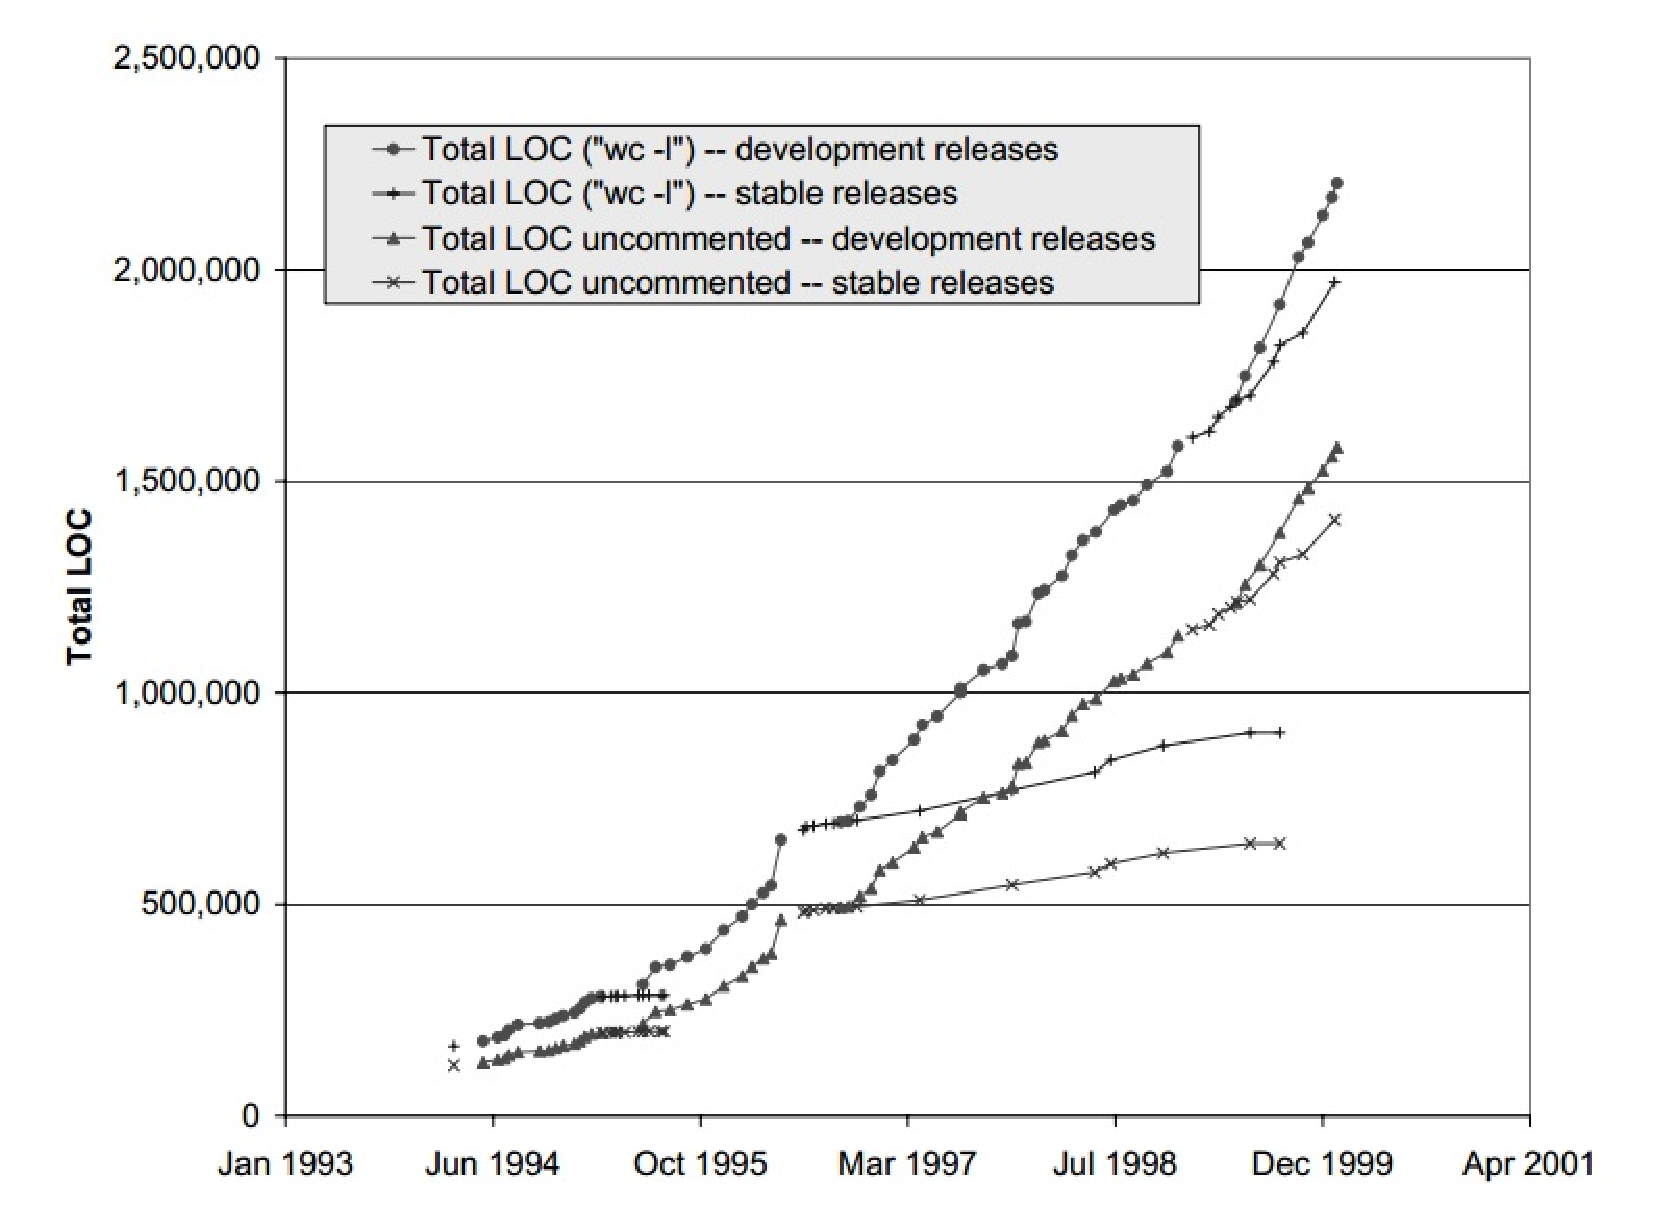
\includegraphics[width=0.6\textwidth]{linux-evolution}
\caption{Evolução do sistema operacional Linux, extraído de \cite{godfrey2000evolution}}
\label{fig-evolucaolinux}
\end{figure}

Os dados presentes no gráfico, até o início dos anos 2000, vão de encontro à quinta lei de Lehman, citada na Tabela \ref{tab-leis-lehman}. No gráfico, o número de linhas de código (LOC) do kernel do sistema, possui taxa de crescimento positiva, enquanto a lei afirma que ao longo do tempo a taxa de crescimento tende a diminuir.
%
Por outro lado, neste trabalho, não estamos tratando a evolução de software apenas do ponto de vista da inserção de novas funcionalidades, o que pode levar ao crescrimento de número de linhas de código, como exemplificado acima. Estamos tratando a evolução de um software livre real, do ponto de vista da sua arquitetura, de acordo com as decisões julgadas pelo seus principais desenvolvedores, conforme descrito nas respostas ao questionário apresentado no Apêndice \ref{form-pesquisa}, para poderem evoluir o projeto de uma forma mais rápida e objetivando formação de uma comunidade de desenvolvedores.

\section{Evolução da Arquitetura}

\subsection{Arquitetura de Software}

%Contexto
%O desenvolvimento de um sistema de software não é uma tarefa simples por conta da complexidade envolvida no processo. Além de lidar com a complexidade inerente ao problema a ser resolvido, devemos nos preocupar em como o software resolve esse mesmo problema. Por esse motivo muitos softwares fracassam, seja por custar muito acima do orçamento, estarem imcompletos ou não solucionarem os problemas como deveriam. Assim um software além de resolver o problema, deve resolvê-lo da forma esperada, satisfazendo atributos de qualidade \cite{germoglio2010fundamentos}.


%Definição
Desde a primeira referência em um relatório técnico intitulado \textit{Software Engineering Tecnhiques} \cite{buxton1970software}, na década de 1970, diversos autores buscaram definir o termo arquitetura de software de software.
%
Mary Shaw e David Garlan \cite{shaw1996software}, Philippe Kruchten, Grady Booch, Kurt Bittner, e Rich Reitman afirmam que: Arquitetura de Software engloba o conjunto de decisões significativas sobre a organização de um sistema de software incluindo: i) seleção de elementos estruturais e suas interfaces pelos quais um sistema é composto; ii) comportamento como especificado em colaboração entre esses elementos; iii) composição dos elementos estruturais e comportamentais dentro de um subsistema maior; iv) um estilo arquitetural que orienta essa organização. Arquitetura de Software também envolve funcionalidade, usabilidade, flexibilidade, desempenho, reuso, compreensibilidade, restrições econômicas e tecnológicas, vantagens e desvantagens, além de preocupações estéticas.
%Definição da ISO 1471
Com o intuito de estabelecer um padrão sobre o que é e para que serve a arquitetura de software, a ISO 1471 estabelece que Arquitetura de Software é a organização fundamental de um sistema incorporada em seus componentes, seus relacionamentos com o ambiente, e os princípios que conduzem seu design e evolução.
%Elementos básicos
Em suma, há três conceitos citados por todos os autores quando se trata de arquitetura de software \cite{dias2000software}:

\begin{itemize}
\item Elementos estruturais ou de software, também chamados de módulos ou componentes, são as abstrações responsáveis por representar as entidades que implementam funcionalidades especificadas.
\item Interfaces ou relacionamentos, também chamados de conectores, são as abstrações responsáveis por representar as entidades que facilitam a comunicação entre os elementos de software.
\item Organização ou configuração que consiste na forma como os elementos de software e conectores estão organizados.
\end{itemize}

%Atributos de qualidade
Durante a especificação da arquitetura é importante ter a atenção nos relacionamentos entre seus elementos. Essas relações especificam a comunicação, o controle da informação e o comportamento do sistema. Consequentemente, essas relações impactam nos atributos de qualidade, sejam os percebidos pelos usuários, ou apenas pelos desenvolvedores \cite{germoglio2010fundamentos}.
%
Os atributos de qualidade são uma das principais preocupações da arquitetura. Eles representam a maneira que o sistema executará suas funcionalidades e são impostos pelos diversos envolvidos no sistema. Podem ser de três tipos:

\begin{itemize}
\item Atributos de produto ditam como o sistema irá se comportar. Exemplos clássicos são: desempenho, disponibilidade, manutenbilidade, escalabilidade, disponibilidade e portabilidade;
\item Atributos organizacionais são padrões ou regras impostas por organizações envolvidas para satisfazer determinados requisitos. 
\item Atributos externos são leis impostas sobre softwares ou requisitos de interoperabilidade entre sistemas.
\end{itemize}

%TODO: referência

%Decisões Arquiteturais
%TODO: referência
Para satisfazer esses atributos a arquitetura não pode ter suas estruturas definidas aleatoriamente. É necessário que o engenheiro de software opte por alternativas, divida o sistema em elementos e defina seus relacionamentos para alcançar os atributos de qualidade desejados. Esse conjunto de decisões é conhecido por decisões arquiteturais.
%Rastreabilidade
%TODO: referência
Qualquer software possui arquitetura, independente dela ser documentada ou projetada. Entretando, uma arquitetura apenas implementada, ou seja, arquitetura sem projeto, não fornece benefícios ou vantagens que uma arquitetura projetada e bem documentada pode oferecer. Entre os benefícios da documentação da arquitetura estão: i) arquitetura como ferramenta de comunicação entre os participantes do projeto; ii) um método ou modelo para a análise antecipada do sistema a ser desenvolvido; iii) ferramenta de rastreabilidade entre os requisitos e os elementos que compõem o sistema, o que é de grande relevância dada a volatilidade dos requisitos durante o processo de desenvolvimento.
%
Além da participação no desenvolvimento e o estudo da nova arquitetura do Mezuro,
neste trabalho, também colaboraremos com documentação de sua arquitetura, e de modo
que possa ser mantida de acordo com as práticas das comunidades de software livre,
ou seja, também mantida e distribuida junto ao código no seu repositório.


%-----------------------parágrafos desconexos---------------------------------------%
% TODO: reescrever por está blabla...
%Por relacionar atributos de qualidade (requisitos não-funcionais) a elementos arquiteturais as decisões auxiliam o rastreameto de requisitos.

%Analisando o ciclo de desenvolvimento de software, é observado que a arquitetura é uma abordagem empregada desde as fases iniciais do processo. Neste instante o nível de abstração da arquitetura é bastante elevado, tendo o objetivo de definir e apresentar a solução computacional que será implementada, auxiliando a tomada de decisões dos stakeholders ou envolvidos no processo de desenvolvimento. Contudo, ao longo do desenvolvimento do software, a arquitetura sofre refinamentos que diminuem o nível de abstração e permitem, por exemplo, a representação dos relacionamentos entre os elementos arquiteturais e os arquivos de código fonte responsáveis por implementá-los \cite{clements2002documenting}.
%---------------------------------------------------------------------------------------%

\subsection{O arcabouço Ruby on Rails}

O Ruby on Rails é um \textit{arcabouço}, disponível como software livre, criado em 2003 por David Heinemeier Hansson.
%
Sua primeira versão foi lançada em 2004, e desde então seu desenvolvimento e utilização são cada vez maiores.
%
Diversos programadores e empresas em todo mundo utilizam esse arcabouço para construirem suas aplicações. Entre as mais conhecidas estão o Twitter (nas primeiras versões), GitHub e Groupon. 
%
O Rails utiliza a linguagem de programação Ruby, criada no Japão em 1995 por Yukihiro "Matz" Matsumoto. A linguagem Ruby é interpretada, multiparadigma, com tipagem dinâmica e gerenciamento de memória automático. O Rails é basicamente uma biblioteca Ruby ou \textit{gem} e é construído utilizando o padrão arquitetural \textbf{MVC}.

Um de seus fundamentos é facilitar o desenvolvimento. O Rails utiliza diversos princípios para orientá-lo do "modo certo" ("Rails way"), possibilitando concentrar esforços no problema do cliente, poupando a equipe do esforço de organizar a estrutura da aplicação a qual é feita pelo arcabouço. Alguns princípios são:

\begin{itemize}

\item \textbf{DRY} - “Don’t Repeat Yourself” - Propõe que um mesmo trecho ou porção de
conhecimento em um código deve possuir representação única no sistema, livre de
redundância e repetições. Quando aplicado, esse princípio possibilita que uma alteração
seja feita em um único local no código, evitando “bad smells” como código duplicado e
facilitando a manutenbilidade do sistema.

\item \textbf{Convenção ao invés de Configuração} (Convention over configuration)- Considerado um paradigma de design que visa diminuir o número de decisões que os desenvolvedores precisam tomar, ganhando simplicidade, sem perder simplicidade.

\item \textbf{REST} - É um estilo arquitetural para aplicações web. O termo REST é um acrônimo para \textbf{RE}presentaional \textbf{S}tate \textbf{T}ransfer. Propõe princípios (não exclusivos ao REST) que definem como Web Standards como HTTP e URIs devem ser usados. Os princípios são:

  \begin{itemize}

  \item Todos os recursos devem ter um identificador. Um conceito comum para identificador na web é a URI;

  \item Utilize links (hipermídia) para referenciar recursos;

  \item Utilize os métodos padrão - São eles GET, POST, PUT, DELETE. Os métodos GET e PUT e DELETE são idempotentes, ou seja, há garantia de que podemos enviar a requisição novamente. Quando emitimos um GET, por exemplo, e não recebermos resposta, não saberemos se a requisição foi perdida ou a resposta que se perdeu. Mas nesse caso podemos simplesmente enviar a solicitação novamente;

  \item Múltipla representação de recursos - diversos formatos dos recursos para diferentes necessidades, como formatos XML, HTML. Isso faz com que seus recursos sejam consumidos não apenas pelo seu aplicativo, mas também por qualquer navegador web;

  \item Comunicação sem estado - Um servidor não deveria guardar o estado da comunicação de qualquer um dos clientes que se comunique com ele além de uma única requisição. A razão para isso é escalabilidade - o número de clientes que podem interagir com o servidor seria consideravelmente impactado se fosse preciso manter o estado do cliente;

  \end{itemize}
\end{itemize}

%TODO: não tem nenhuma referência para nada o que você falou até aqui...
% Não foi você que inventou isso tudo, tem que dar o crédito a quem definiu ;)

%---------------------------------------------------------------------------------------%
%Essa seção é importante pois a evolução do Rails foi um dos motivos que motivou a evolução da plataforma Mezuro.
\textbf{Evolução do Ruby on Rails}

O arcabouço Rails, desde seu lançamento, sofre frequentes alterações, e com isso novas versões são lançadas constantemente, conforme apresentado na Tabela~\ref{tab:rails_versions}. Muitos desenvolvedores enxergam essas constantes mudanças como um ponto negativo, ao passo que há incompatibilidade de algumas "gems" de uma versão para outra. Por outro lado, outros aprovam essa característica pois a cada atualização há melhora no produto, com adição de novos recursos, além de ser um incentivo para a implementação de testes, já que eles auxiliam a manter a integridade da aplicação a cada atualização.

\begin{table}[H]
\begin{center}
    \begin{tabular}{ | l | l |}
    \hline
    Versão & Data \\ \hline
    1.0 & 13/12/2005 \\ \hline
    1.2 & 19/01/2007 \\ \hline
    2.0 & 7/12/2007 \\ \hline
    2.1 & 01/06/2008 \\ \hline
    2.2 & 21/11/2008 \\ \hline
    2.3 & 16/03/2009 \\ \hline
    3.0 & 29/08/2010 \\ \hline
    3.1 & 31/08/2011 \\ \hline
    3.2 & 20/01/2012 \\ \hline
    4.0 & 25/06/2013 \\ \hline
    \end{tabular}
    \caption{Versões do Rails}
    \label{tab:rails_versions}
\end{center}
\end{table}

Entre os novos recursos oferecidos pela versão 4 do Rails, que é a versão usada no novo Mezuro, estão:

\begin{itemize}

	\item Páginas mais rápidas através da utilização de Turbolinks. Ao invés de deixar o navegador recompilar o JavaScript e CSS entre cada mudança de página, a instância da página atual é mantida, substituindo apenas o conteúdo e o título.

	\item Suporte para a expiração de cache baseado em chave, que automatiza a invalidação do cache e deixa mais fácil a implementação de estruturas de cache sofisticadas.

	\item Streaming de vídeo ao vivo em conexões persistentes.

	\item Melhorias no ActiveRecord para aprimorar a consistência do escopo e da estrutura das queries.

	\item Padrões de segurança locked-down.

	\item Threads seguras por padrão e a eliminação da necessidade de configurar servidores com thread.

\end{itemize}

%TODO: também se referencia ou coloca-se uma nota de rodapé de onde o leitor pode ver isso e conhecer mais a tecnologia.

É importante discutir sobre a evolução deste arcabouço pois esse foi um dos motivos que motivaram a evolução da plataforma Mezuro. Isso para aproveitar os recursos mais novos disponíveis nas versões mais recentes, além de desfrutar de maior suporte da comunidade deste arcabouço como da linguagem utilizada por ele, a linguagem Ruby. Um questionário com questões relacionadas a evolução do Mezuro se encontra no Apêndice\ref{form-pesquisa} deste documento e respostas de alguns dos colaboradores  se encontram no Anexo\ref{resp-pesquisa}.

%---------------------------------------------------------------------------------------%

\textbf{Padrão Arquitetural MVC}

O padrão \textbf{MVC} começou como um arcabouço desenvolvido por Trygve Reenskaug para a plataforma SmallTalk, no final dos anos 70. Desde então, ele exerce grande influência sobre diversos arcabouços que promovem interação com usuário, como é o caso do Ruby on Rails.
%
O MVC visa separar a representação da informação da interação com o usuário. Para atingir esse objetivo são utilizados três ``papéis'', conforme apresentado do na Figura~\ref{fig:mvc}:
%
(i) O modelo (\textit{model}) que representa informações do domínio, como dados
da aplicação, regras de negócio, lógica e funções;
%
A visão (\textit{view}) que são saídas de representação dos dados do modelo ao
usuário. Um exemplo comum de visão é uma pagína HTML contendo dados presentes
no modelo.
%
O útimo papel, o controlador (\textit{controller}) é responsável por receber
requisições da visão, manipula-las, utilizando dados do modelo, e atualizar a
visão para satisfazer as requisições do usuário.

\graphicspath{{figuras/}}
\begin{figure}[H]
\centering
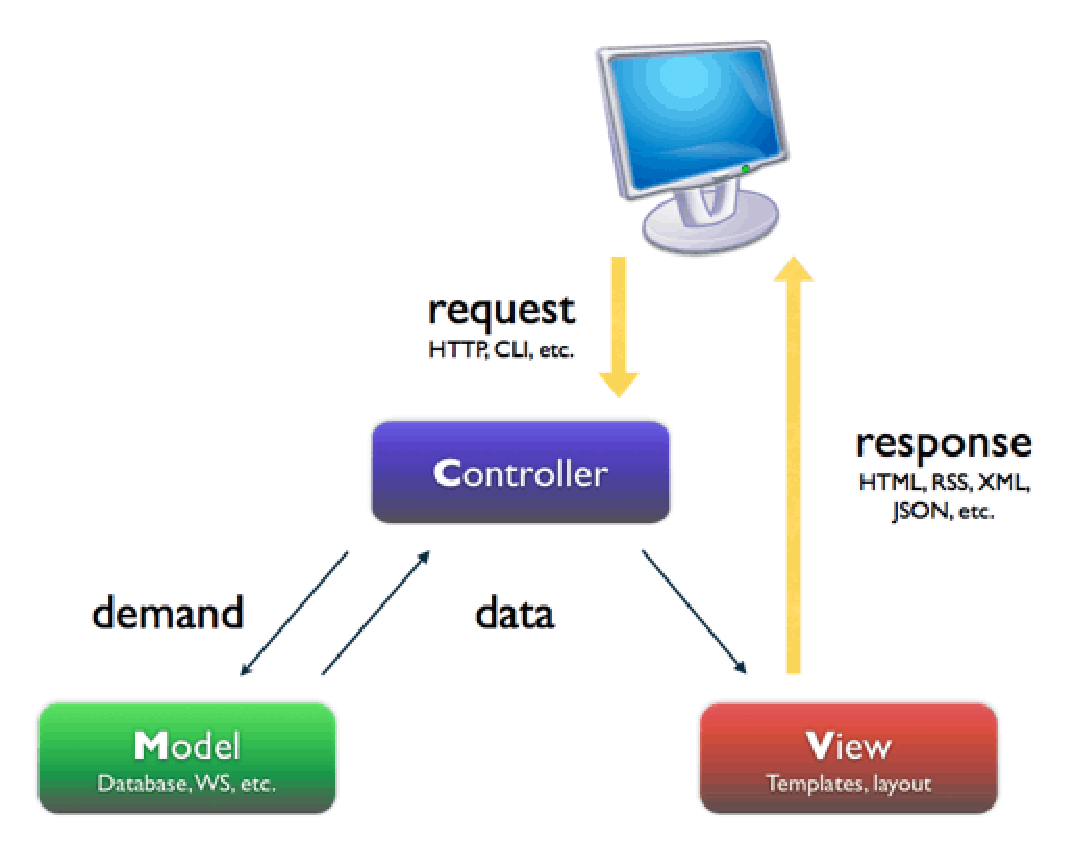
\includegraphics[width=0.5\textwidth]{mvc}
\caption{Representação do padrão MVC}
\label{fig:mvc}
\end{figure}

O exemplo abaixo ilustra um cenário de execução de uma funcionalidade com o padrão MVC.

\begin{mdframed}[frametitle={Exemplo},roundcorner=5pt]
Um usuário navega em um site de vendas de veículos. Ao pressionar o botão para visualizar determinado veículo, o navegador carrega a página de detalhes e a devolve ao usuário. Esse processo começa quando na VIEW o usuário pressiona o botão de visualização. A URL gerada é processada por um método da CONTROLLER de veículos. Esse método solicita ao MODEL o veículo correspondente a URL, então a VIEW é renderizada com os dados do veículo correspondente, obtidos pela CONTROLLER.
\end{mdframed}

%TODO: tudo sem referência até aqui...

%---------------------------------------------------------------------------------------%

\textbf{Arquitetura do Rails}

Entre os elementos da arquitetura de software, há elementos estáticos e dinâmicos. Elementos estáticos definem as partes de um sistema e sua organização. Entre elementos estáticos estão: i) elementos de software; ii) elementos de dados; iii) elementos de hardware. 
%
As características do Rails estão distribuídas entre elementos, conforme ilustrado na Figura~\ref{fig:rails-architecture}.
%
Os relacionamentos entre os elementos também estão inclusos, e também compõem o aspecto estático da arquitetura do sistema \cite{germoglio2010fundamentos}.
%
Já os elementos dinâmicos definem o comportamento do sistema e representa o sistema em execução. Nele estão incluídos processos, protocolos, módulos e classes que realizam comportamento.

\graphicspath{{figuras/}}
\begin{figure}[H]
\centering
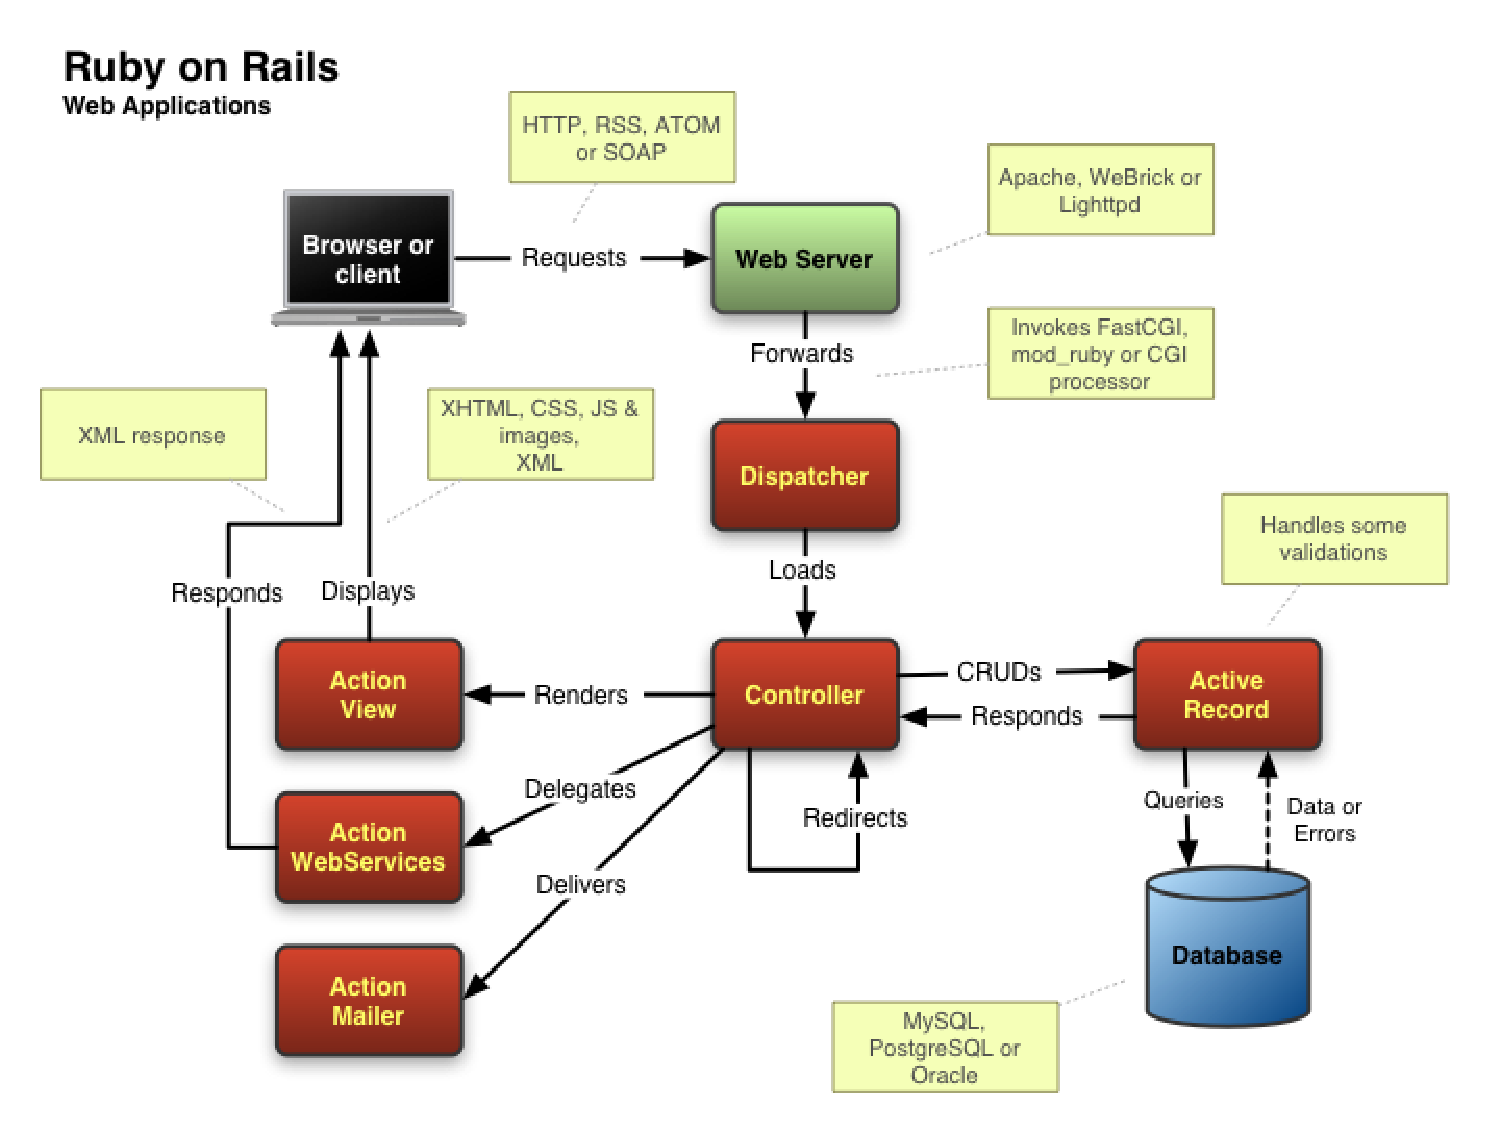
\includegraphics[width=0.7\textwidth]{rails-overview}
\caption{Interação entre os componentes do Rails. Extraído  de \cite{mejia2011rails}}
\label{fig:rails-architecture}
\end{figure}


\begin{enumerate}

	\item \textbf{Action Mailer} fornece a capacidade de criação de serviços de e-mail. Podendo enviar e-mails baseados em templates adaptáveis ou receber e processar um e-mail;

	\item \textbf{Action Pack} é composto por: \\

	\begin{description}
 
	\item [Action Controller] é o componente que gerencia os controllers em uma aplicação Rails. Ele processa as requisições que chegam de uma aplicação Rails, recebe seus
parâmetros e os envia para as ações pretendidas;

	\item [Action View] gerencia as views da aplicação. Isto é, as saídas HTML e XML por 	padrão. Gerencia a renderização de templates aninhados ou parciais , e inclui suporte
embutido para AJAX;

	\end{description}

\item \textbf{Active Record} é abase dos \textit{models}. Ele fornece a independência de banco de dados e CRUD básico. Ele é utilizado para criar a representação, em orientação a objetos, dos
dados presentes no banco de dados;

\item \textbf{Active Resource} gerencia conexões entre objetos de negócio e serviços web RESTful.
Ele mapeia recursos baseados em web para objetos locais com lógica CRUD;

\item \textbf{Active Support} uma coleção de classes de utilidade e extenções da biblioteca padrão do
Ruby que são utilizadas pelo Rails, tanto em seu núcleo quanto para suas aplicações;

\item \textbf{Railties} é o núcleo do código Rails e é ele quem constrói novas aplicações Rails e junta os diversos componentes;

\end{enumerate}


%TODO: concluir algo














